\documentclass[landscape]{article}
\usepackage {lscape} 
\usepackage[letterpaper,margin=1.5cm]{geometry}
\usepackage{lipsum,multicol}
\usepackage{graphicx} 
\begin{document}
\begin{multicols}{3}

\subsection*{Software utilizado en el mantenimiento}

La utilizaci\'on de software para el mantenimiento del disco duro en buen estado y obtner el m\'aximo rendimiento de \'el, son aspectos necesarios para guardar de manera segura la informaci\'on. Existe una amplia variedad de programas de software que se encargan de estas tareas.  Por lo que a continaci\'on se describir\'a como funcionan los programas m\'as importantes para el mantenimiento del disco y la revisi\'on del sistema.

\subsection*{Herramientas de optimizaci\'on}

Un optimizador es una utiler\'ia de software relativamente amplia que puede incluir diversas caracter\'isticas y funciones. Por lo general los optimizadores de deisco est\'an dise\~nados para manejar la informaci\'on guardada en la computadora.

*{\bf Liberador de espacio.}

Liberador de espacio en disco busca en la unidad y enumera los archivos temporales, archivos de cach\'e de Internet y archivos de programa innecesarios que puede eliminar de forma segura.

*{\bf Desfragmentador.}

La desfragmentaci\'on sucede despu\'es de que el sistema operativo ha escrito diferentes versiones de los archivos varias veces, esto es, un archivo despu\'es de ser modificado al guardarse no ocupa direcciones de memoria contiguas en el disco duro, el desfragmentador se ocupa de acomodar los archivos en direcciones de memoria contiguas.

*{\bf Scandisk.}

Revisa la estructura de archivos, directorios y la superficie del disco que se le indique. Esta se encuentra dentro de las herramientas del sistema y puede efecuar una revisi\'on de estructura y de superficie f\'isica (l\'ogica) del disco.


\columnbreak

\vspace*{10cm}
\section*{Grupo No. 34}
\vspace*{1cm}
\subsection*{Integrantes}
\vspace*{0.5mm}
\begin{center}
\begin{tabular}{|l||c|} \hline
Primer Integrante & 2016-00000 \\
Segundo Integrante & 2016-00001 \\ 
Siguiente Integrante & 2016-00002 \\ \hline
\end{tabular}
\end{center}
\columnbreak


\part*{\centerline{\bf GU\'IA R\'APIDA}}
\vspace*{1in}
\part*{\centerline{\bf MANTENIMIENTO}}
\vspace*{1cm}
\part*{\centerline{\bf DE UN}}
\vspace*{1cm}
\part*{\centerline{\bf ORDENADOR}}

\bigskip

\begin{center}
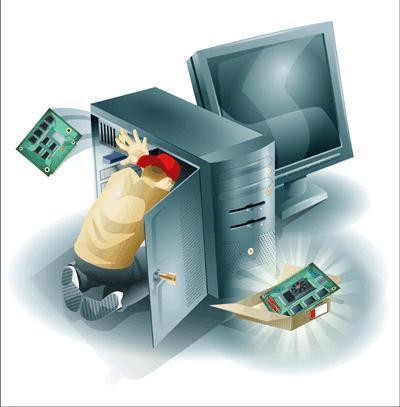
\includegraphics[height=50mm]{Compu1.jpg}
\end{center}

\end{multicols}
\end{document}